\subsubsection{Adapted SAGAT}
\label{subsubsec:results_adapted_sagat_2}

Figures \ref{fig:boxplot_sagat_4_scene} and \ref{fig:boxplot_sagat_4_rounds} bring the boxplots. According to Figure \ref{fig:boxplot_sagat_4_scene}, both groups presented a higher situation awareness with ‘mixture’ and ‘haptic’. On the other hand, Figure \ref{fig:boxplot_sagat_4_rounds} confirms that the difference between the rounds is more significant for blind participants. 

\begin{figure}[!htb]
    \centering
    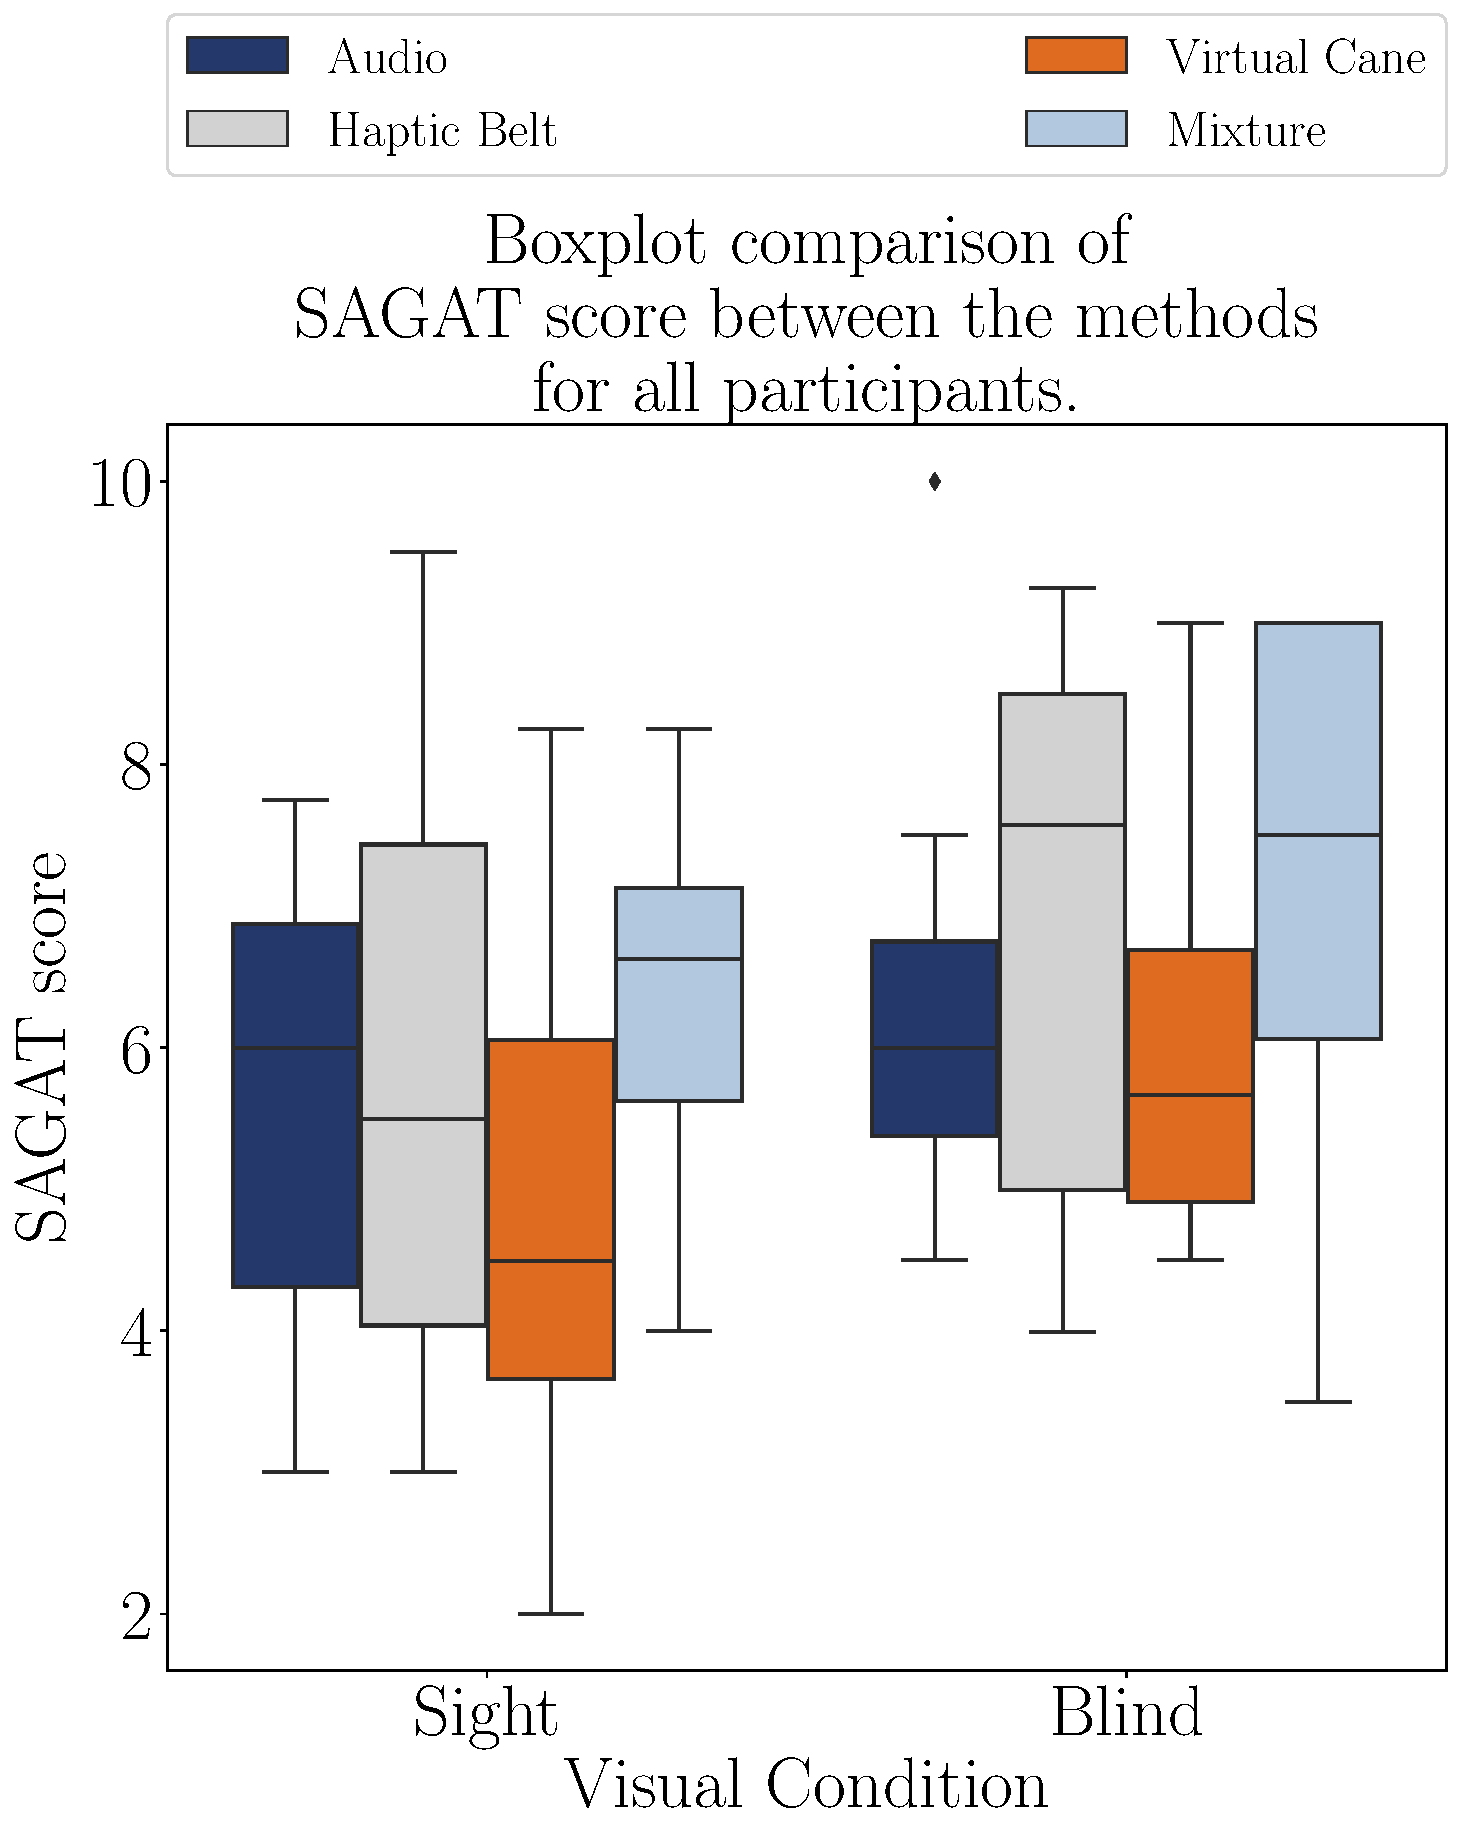
\includegraphics[width = 0.75\linewidth]{3 - Resultados//Figuras/boxplot_sagat_4_scene.pdf}
    \caption{Boxplot of the SAGAT score of the participants grouped by the methods.}
    \label{fig:boxplot_sagat_4_scene}
\end{figure}
\begin{figure}[!htb]
    \centering
    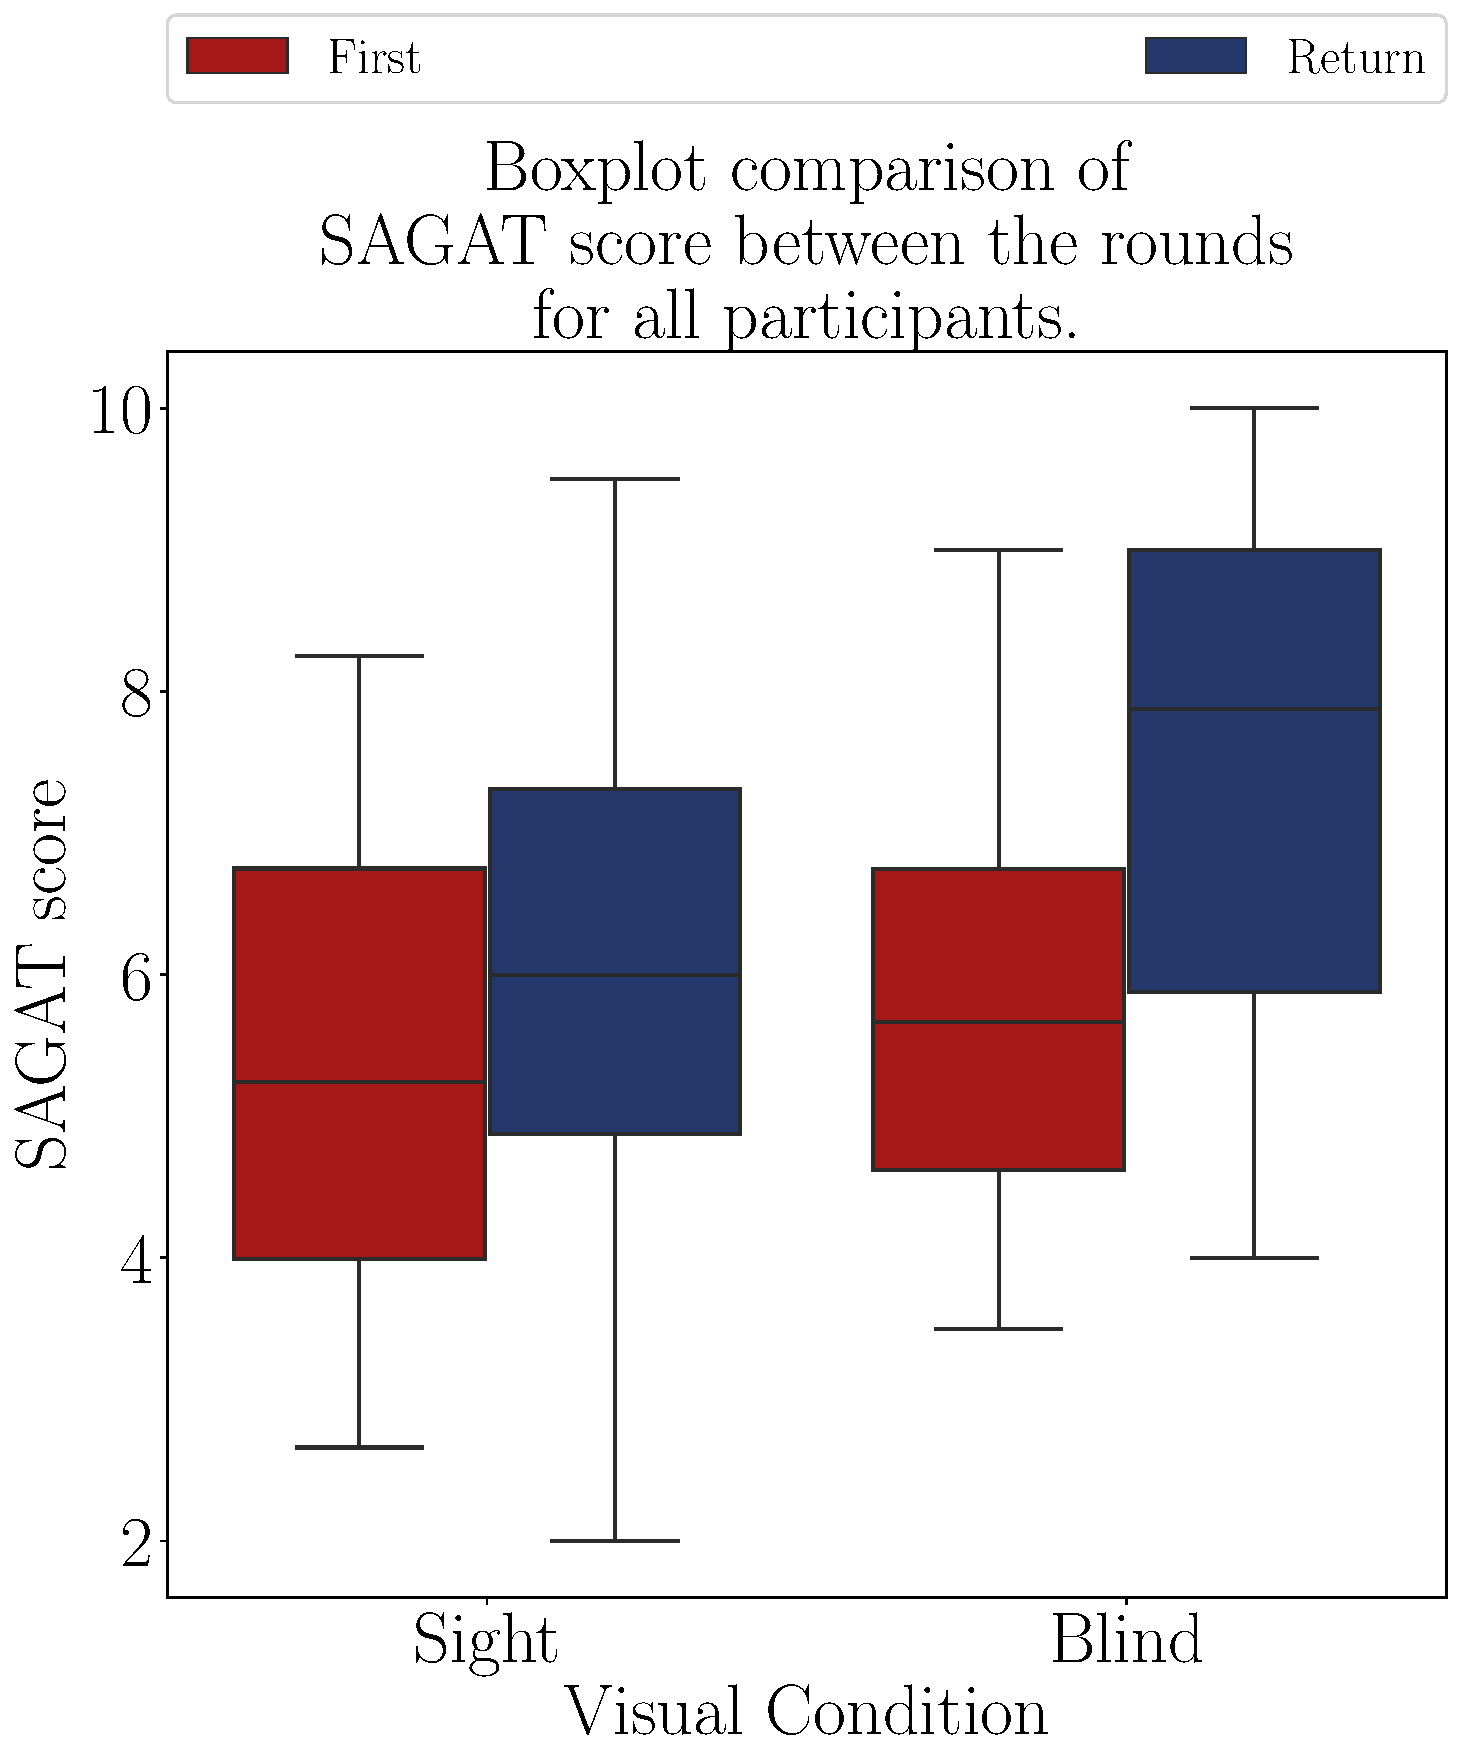
\includegraphics[width = 0.75\linewidth]{3 - Resultados//Figuras/boxplot_sagat_4_rounds.pdf}
    \caption{Boxplot of the SAGAT score of the participants grouped by the rounds.}
    \label{fig:boxplot_sagat_4_rounds}
\end{figure}

The variance of the residuals is not equal among the participants. Table \ref{tab:blocanova_sagat_avg_two_way_blind_sight} brings the p-value from ANOVA. While for the blind participants, the rounds are a significant factor and the methods are not, for the sighted participants the result is the opposite, showing a significant influence of the methods and not of the rounds.

\begin{table}[!htb]
    \caption{Anova p-value for the SAGAT score on each method}
    \label{tab:blocanova_sagat_avg_two_way_blind_sight}
\begin{minipage}{0.45\linewidth}
    \subcaption{Blind participants}
    
\centering
\begin{tabular}{ll}
\toprule
          Source & P-Value \\
\midrule
    \    Methods &   0.277 \\
     \    Rounds & 0.002** \\
\    Interaction &   0.834 \\
\bottomrule
\end{tabular}

\end{minipage}%
\begin{minipage}{0.05\linewidth}
    \hfill
\end{minipage}%
\begin{minipage}{0.45\linewidth}
    \subcaption{Sight participants}
    
\centering
\begin{tabular}{ll}
\toprule
          Source & P-Value \\
\midrule
    \    Methods & 0.035** \\
     \    Rounds &   0.095 \\
\    Interaction &   0.578 \\
\bottomrule
\end{tabular}
    
\end{minipage}
\end{table}